\chapter{Implementacja aplikacji}
%
\section{Architektura aplikacji webowej}
Aplikajca składa się z następujących elementów:
\begin{itemize}
    \item Mongodb - baza danych
    \item Redis \cite{redis} - przechowywanie JWT (ang. \textit{JSON Web Token}) \cite{jwt} tokenów po wylogowaniu
    \item Go - część serwerowa napisana w języku Go
    \item Android - aplikacja mobila
    \item Docker - kontener dla wdrożenia aplikacji webowej
\end{itemize}
\begin{figure}[ht]
    \centering
        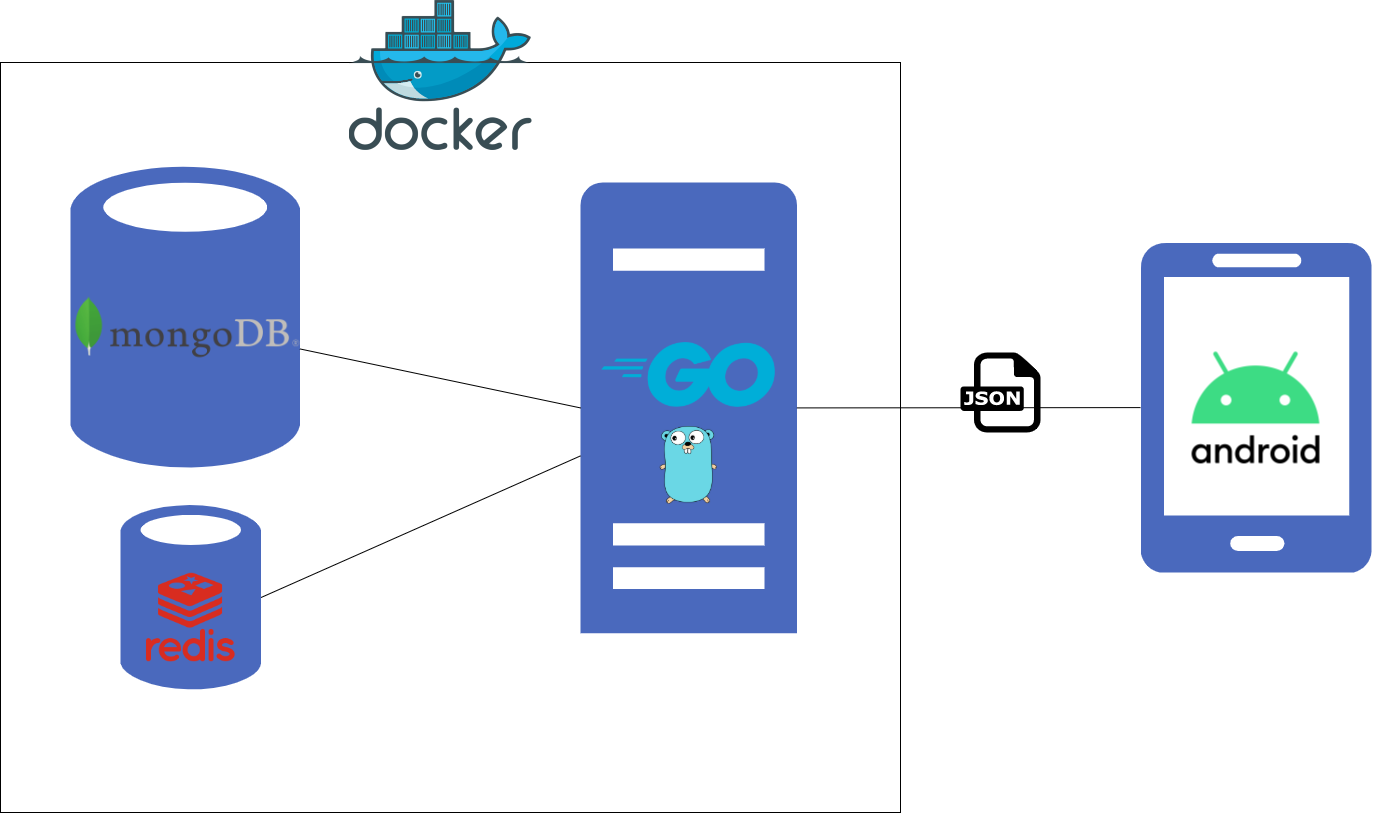
\includegraphics[width=0.8\linewidth]{rys03/system_architecture_diagram.png}
        \caption{architektura systemu \cite{diagrams_net}}
    \label{fig:system architecture diagram}
\end{figure}
\section{Model bazy danych}
\section{Implementacja części serwerowej}
\subsection{Struktura RestApi}
\subsubsection{Struktura plików RestApi}
\subsubsection{Przepływ danych}
\subsubsection{Nażędzia i technologie}
\subsubsection{Punkty końcowe}
\subsection{Funkcje części serwerowej}
\subsubsection{Użytkownik}
\paragraph{Dodawanie}
\paragraph{Wczytywanie}
\paragraph{Edycja}
\paragraph{Usunięcie}
\subsubsection{Autentykacja / Logowanie i rejestracja}
\subsubsection{Stacja}
\paragraph{Dodawanie}
\paragraph{Wczytywanie}
\paragraph{Edycja}
\paragraph{Usunięcie}
\subsubsection{Komentarz}
\paragraph{Dodawanie}
\paragraph{Wczytywanie}
\paragraph{Edycja}
\paragraph{Usunięcie}
%
\section{Implementacja Intefejsu użytkownika}
\subsection{Struktura AndroidUI}
\subsubsection{Struktura plików AndroidUI}
\subsubsection{Przepływ danych}
\subsubsection{Nażędzia i technologie}
\subsection{Funkcje aplikacji mobilnej}
\subsubsection{Autentykacja / Logowanie i rejestracja}
\subsubsection{Stacja}
\paragraph{Dodawanie}
\paragraph{Wczytywanie}
\paragraph{Edycja}
\subsubsection{Komentarz}
\paragraph{Dodawanie}
\paragraph{Wczytywanie}
